
%(BEGIN_QUESTION)
% Copyright 2015, Tony R. Kuphaldt, released under the Creative Commons Attribution License (v 1.0)
% This means you may do almost anything with this work of mine, so long as you give me proper credit

Examine this differential current protection system for a transformer, supplying three-phase power to a feeder from a substation bus:

$$\includegraphics[width=15.5cm]{i02563x01.eps}$$

\vskip 10pt

Suppose the cable connecting feeder phase 2's CT to the 87-2 relay fails shorted, such that the relay no longer senses current from the secondary winding of the transformer through that phase.  Will the other two differential current relays continue to provide adequate protection for the transformer?  Explain why or why not, in detail.

\vfil 

\underbar{file i02563}
\eject
%(END_QUESTION)





%(BEGIN_ANSWER)

This is a graded question -- no answers or hints given!

%(END_ANSWER)





%(BEGIN_NOTES)

With one CT circuit failed ({\it any} one for that matter!), the corresponding 87 relay will immediately detect an imbalanced current condition for any amount of line current and trip the circuit breaker as designed.  To put it simply, the system will falsely trip and refuse to operate.

%INDEX% Protective relay: differential current (87)

%(END_NOTES)


